
\documentclass{FMTslides}
\usepackage[labelformat=simple]{subfig}
\renewcommand{\thesubfigure}{\relax} 
\pdfpageattr {/Group << /S /Transparency /I true /CS /DeviceRGB>>}

\title[Model-based Testing with Graph Grammars]{Model-based Testing with Graph Grammars}
\conference{\!\!\!M.Sc. Colloquium}
\author{Vincent de Bruijn}
\institute{Formal Methods and Tools, Faculty of EECMS \\ University of Twente, The Netherlands}
\date{September 4th, 2012}

%%%% END ARROWS %%%%%%%%%%%%%%%%%%%%%%%%%

%%%%%%%%%%%%%% TIKZ %%%%%%%%%%%%%%%%
\tikzstyle{background rectangle}= [rounded corners, fill=yellow!20, draw=black, rounded corners=1ex]
\tikzstyle{every picture}=[show background rectangle, ->,>=latex,auto,node distance=1.3cm,thick,initial text=,initial where=above,scale=0.8,transform shape]
\tikzstyle{every state}=[draw=yellow!20,line width=4pt,fill=black,minimum size=5pt]

\tikzstyle{loop right}=[in=-30,out=30,looseness=8]
\tikzstyle{loop left}=[in=150,out=210,looseness=8]
\tikzstyle{loop above}=[in=60,out=120,looseness=8]
\tikzstyle{loop below}=[in=240,out=300,looseness=8]

\tikzstyle{loop above right}=[in=5,out=65,looseness=8]
\tikzstyle{loop above left}=[in=105,out=165,looseness=8]
\tikzstyle{loop slightly above left}=[in=125,out=185,looseness=8]
\tikzstyle{loop slightly above right}=[in=5,out=65,looseness=8]
\tikzstyle{loop below left}=[in=195,out=255,looseness=8]
\tikzstyle{loop below right}=[in=285,out=-15,looseness=8]
\tikzstyle{loop slightly below left}=[in=155,out=215,looseness=8]
\tikzstyle{loop slightly below right}=[in=305,out=5,looseness=8]

\tikzstyle{nodeSmall} = [state, node distance=1.5cm, draw=yellow!20, fill=black]
\tikzstyle{finalNode} = [node distance=1.5cm]
\tikzstyle{onEdge}=[fill=yellow!20, pos=0.5]
%%%%%%%%%%%%%% END TIKZ %%%%%%%%%%%%%

\AtBeginSection[]
{
  \begin{frame}
    \frametitle{Inhoudsopgave}
    \tableofcontents[currentsection]
  \end{frame}
}

\begin{document}

\maketitleslide

\section*{Introduction}

\begin{frame}{Model-based Testing (1/3)}
\begin{itemize}[<+->]
  \item Why testing?
  \begin{itemize}
    \item List of requirements
    \item Test if implementation satisfies requirements
  \end{itemize}
  \item Creating tests manually:
  \begin{itemize}
    \item Error-prone
    \item Time intensive
  \end{itemize}
  \item Solution
  \begin{itemize}
    \item Create model from the requirements
    \item Generate tests automatically using model
  \end{itemize}
\end{itemize}
\end{frame}

\begin{frame}{Model-based Testing (2/3)}
\begin{block}{Model}
\begin{itemize}
  \item An abstract representation of the behavior of a system
\end{itemize}
\end{block}
\begin{figure}
%%%% END ARROWS %%%%%%%%%%%%%%%%%%%%%%%%%

%%%%%%%%%%%%%% TIKZ %%%%%%%%%%%%%%%%
\tikzstyle{background rectangle}= [rounded corners, fill=yellow!20, draw=black, rounded corners=1ex]
\tikzstyle{every picture}=[show background rectangle, ->,>=latex,auto,node distance=1.3cm,thick,initial text=,initial where=above,scale=0.8,transform shape]
\tikzstyle{every state}=[draw=yellow!20,line width=4pt,fill=black,minimum size=5pt]

\tikzstyle{loop right}=[in=-30,out=30,looseness=8]
\tikzstyle{loop left}=[in=150,out=210,looseness=8]
\tikzstyle{loop above}=[in=60,out=120,looseness=8]
\tikzstyle{loop below}=[in=240,out=300,looseness=8]

\tikzstyle{loop above right}=[in=5,out=65,looseness=8]
\tikzstyle{loop above left}=[in=105,out=165,looseness=8]
\tikzstyle{loop slightly above left}=[in=125,out=185,looseness=8]
\tikzstyle{loop slightly above right}=[in=5,out=65,looseness=8]
\tikzstyle{loop below left}=[in=195,out=255,looseness=8]
\tikzstyle{loop below right}=[in=285,out=-15,looseness=8]
\tikzstyle{loop slightly below left}=[in=155,out=215,looseness=8]
\tikzstyle{loop slightly below right}=[in=305,out=5,looseness=8]

\tikzstyle{nodeSmall} = [state, node distance=1.5cm, draw=yellow!20, fill=black]
\tikzstyle{finalNode} = [node distance=1.5cm]
\tikzstyle{onEdge}=[fill=yellow!20, pos=0.5]
%%%%%%%%%%%%%% END TIKZ %%%%%%%%%%%%%

\begin{tikzpicture}[scale=1.5]
	\tikzstyle{every state}=[draw=black,line width=1pt,fill=white,minimum size=5pt]

	\node[state, initial left] (s0) {\footnotesize $s_0$};
	\node[state] (s1) [right=3cm of s0] {\footnotesize $s_1$};
   	\node[state] (s2) [below=2cm of s1] {\footnotesize $s_2$};
	
	\path        (s0) edge node [auto] {?coin} (s1)
					(s1) edge node [auto] {?button} (s2)
					(s2) edge node [auto] {!coffee} (s0);
\end{tikzpicture}

\end{figure}
\end{frame}

\begin{frame}{Model-based Testing (3/3)}
\begin{figure}
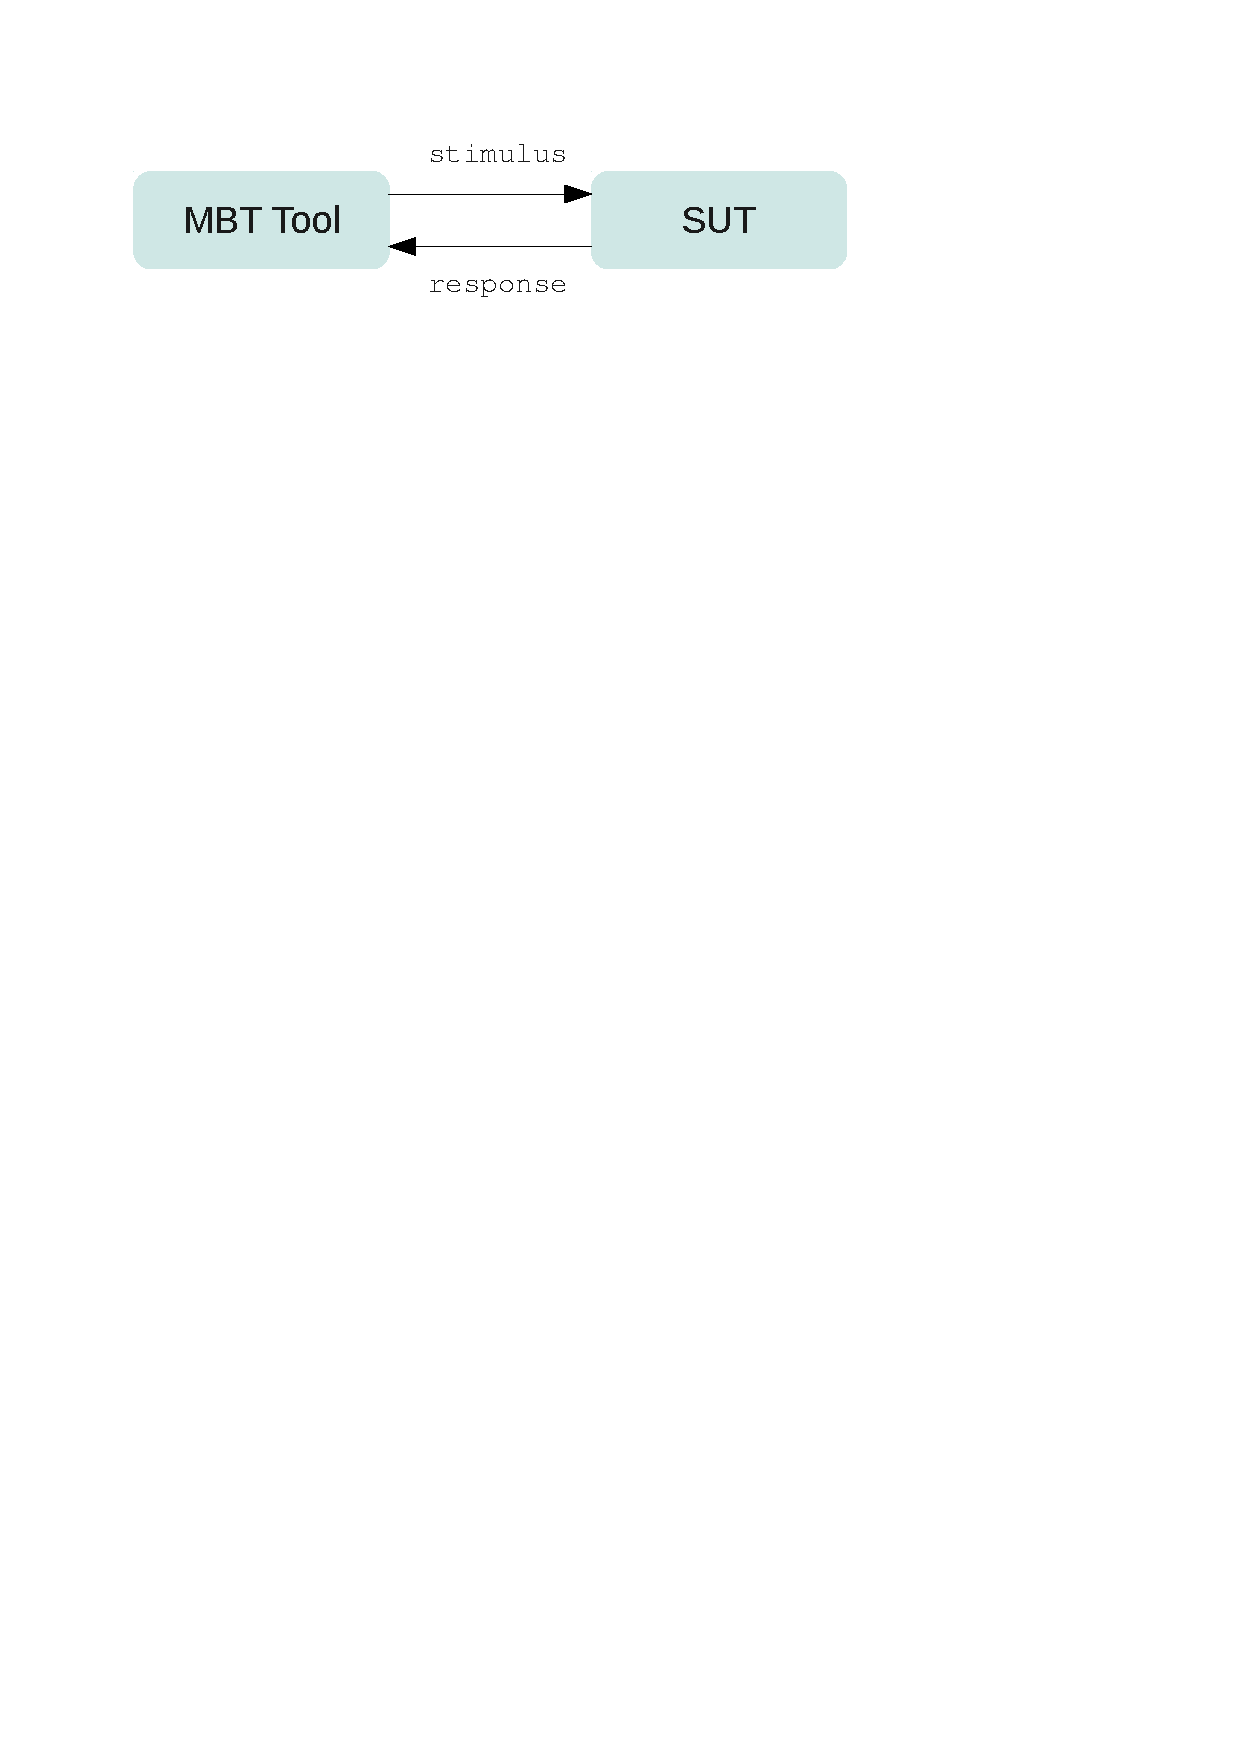
\includegraphics[scale=0.75]{./figures/mbt.pdf}
\end{figure}
\begin{enumerate}[<+->]
\item Take possible input from model
\item Apply input to SUT
\item Observe response(s)
\item Check if according to model
\item Notify tester whether test passed or failed
\item Repeat
\end{enumerate}
\end{frame}

\begin{frame}{Graph Grammars (1/2)}
\begin{figure}
\centering
    \subfloat[before]{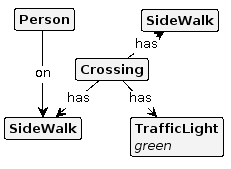
\includegraphics[scale=0.6]{./figures/start.png}}
    \subfloat[after]{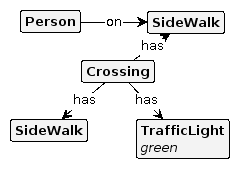
\includegraphics[scale=0.6]{./figures/start1.png}}
\end{figure}

\begin{itemize}[<+->]
  \item Graphs represent system states
  \item Graph rules express possible changes to graph
  \item All possible changes make a \textit{Graph Transition System}
\end{itemize}
\end{frame}

\begin{frame}{Graph Grammars (2/2)}
\begin{figure}
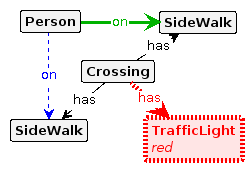
\includegraphics[scale=0.75]{./figures/cross.png}
\end{figure}
\begin{itemize}[<+->]
  \item Black and blue parts have to be present in graph
  \item Red parts may not be present in graph
  \item Blue is erased from graph
  \item Green is added to graph
\end{itemize}
\end{frame}

\begin{frame}{Tools}
\begin{itemize}[<+->]
\item Axini Test Manager (ATM)
\item GRaphs for Object-Oriented VErification (GROOVE)
\end{itemize}
\end{frame}

\begin{frame}{Research Goals)}
\begin{itemize}[<+->]
  \item Goals
  \begin{itemize}
    \item Use GROOVE and ATM to create model-based testing tool with Graph Grammars
    \item Validate this tool using case studies
  \end{itemize}
  \item Motivation
  \begin{itemize}
    \item Graphs are well-known and often used to represent system states
    \item Rules are useful for describing computations
  \end{itemize}
\end{itemize}
\end{frame}

\makecontentsslide

\section[Setup]{Setup}

\begin{frame}{Setup (1/2)}
\begin{itemize}[<+->]
  \item Graphs for humans, transition systems for computers
  \item ATM uses \textit{Symbolic Transition Systems}
\end{itemize}
\begin{figure}
\begin{tikzpicture}
	\tikzstyle{every state}=[draw=black,line width=1pt,fill=white,minimum size=5pt]

	\node[state, initial left] (s0) {\footnotesize $s_0$};
	\node[state] (s1) [right=5cm of s0] {\footnotesize $s_1$};
   	\node[state] (s2) [below=2cm of s1] {\footnotesize $s_2$};
	
	\path        (s0) edge node [auto] {?coin(c) | c=0.20 \/ c=0.50 | C:=c } (s1)
					(s1) edge node [auto] {?button} (s2)
					(s2) edge node [auto] {!coffee | C=0.50 | C:=0} (s0);
\end{tikzpicture}

\end{figure}
\end{frame}

\begin{frame}{Setup (2/2)}
\begin{itemize}[<+->]
  \item The tool:
  \begin{enumerate}
    \item creates STS from the GG in GROOVE
    \item sends STS to ATM
    \item does model-based testing in ATM
  \end{enumerate}
  \item Step number 1 main part of this research.
\end{itemize}
\end{frame}

\section[GG2STS]{From Graph Grammar to STS}

\begin{frame}{Algorithm}
\begin{enumerate}[<+->]
\item Create variables from data values
\item Explore GTS disregarding data values
\item Parse guards and updates from rules
\end{enumerate}
\begin{figure}
\centering
    \subfloat[graph]{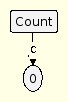
\includegraphics[scale=0.6]{./figures/start-count.png}}
    \subfloat[rule]{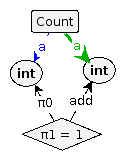
\includegraphics[scale=0.6]{./figures/add.png}}
    \subfloat[STS]{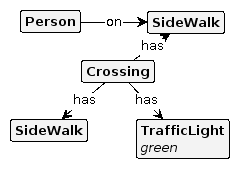
\includegraphics[scale=0.6]{./figures/start1.png}}
\end{figure}
\end{frame}

\begin{frame}{Constraints}
  \begin{enumerate}[<+->]
    \item Variables have to be unique
    \item Variables cannot be part of NACs
    \item Structural constraints on node creating rules
  \end{enumerate}
  one picture here with all mistakes.
\end{frame}

\section[Validation]{Validation}

\begin{frame}{Model Examples}
\begin{itemize}[<+->]
  \item 4 small examples used:
  \begin{enumerate}
    \item a boardgame
    \item a puzzle
    \item a reservation system
    \item a bar tab system
  \end{enumerate}
\end{itemize}
\end{frame}

\begin{frame}{Case study (1/3)}
  \begin{itemize}[<+->]
  \item Self-scan register
\end{itemize}
\begin{figure}
\centering\includegraphics[scale=0.6]{./figures/register.png}
\end{figure}
\end{frame}

\begin{frame}{Case study (2/3)}
  

\begin{figure}
\centering
    \subfloat[graph]{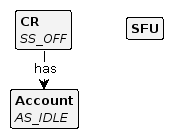
\includegraphics[scale=0.6]{./figures/start-scrp.png}}
    \subfloat[request]{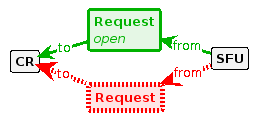
\includegraphics[scale=0.6]{./figures/open.png}}
    \subfloat[response]{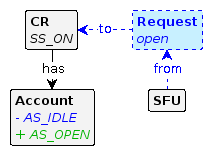
\includegraphics[scale=0.6]{./figures/success.png}}
    \subfloat[error]{\includegraphics[scale=0.6]{./figures/not-signed-in.png}}
\end{figure}
\end{frame}

\section[Conclusion]{Conclusion}

\begin{frame}{Conclusion}
  \begin{itemize}[<+->]
    \item Created a tool for model-based testing with Graph Grammars
    \item Transformation needs to be extended: complex data structures
    \item Modelling behavior with GGs is effective
  \end{itemize}
\end{frame}

\end{document}
